\documentclass[landscape,footrule]{foils}
\usepackage[lecture-serie]{foiltex-extra}
\usepackage{crysymb}
\usepackage{graphics}
\usepackage[pdftex]{graphicx} 




\newcommand{\lecture}{Performance evaluation}
\newcommand{\lserie}{LTAT.02.004 Machine Learning II}
\newcommand{\ldate}{14 February, 2022}
\newcommand{\lauthor}{Sven Laur}
\newcommand{\linst}{University of Tartu}
\graphicspath{{./illustrations/}}
%\MyLogo{\lserie.\  Performance evaluation, \ldate}


\newcommand{\leqm}{\ \leq_m}


\newcommand{\bigvskip}{\vskip 2em}
\newcommand{\lastline}{\vspace*{-2ex}}
\newcommand{\spreadappart}{\vspace*{\fill}}
\renewcommand{\vec}[1]{\boldsymbol{#1}}

\DeclareMathOperator{\supp}{supp}
\DeclareMathOperator{\conf}{conf}
\DeclareMathOperator{\precision}{precision}
\DeclareMathOperator{\recall}{recall}


\newcommand{\fpar}[2]{\frac{\partial#1}{\partial#2}}

\begin{document}
\titlefoil

\foilhead[-0.5cm]{Can we quantify model performance at all?}

\centerline{
\includegraphics[height=4cm]{midjourney_01}\hspace*{0.5cm}
\includegraphics[height=4cm]{midjourney_02}\hspace*{0.5cm}
\includegraphics[height=4cm]{midjourney_03}\hspace*{0.5cm}
}

For some machine learning tasks there is no direct performance measure
\begin{triangles}
\item speech synthesis
\item conversational chat bots
\item image and music generation tasks
\end{triangles}
\vspace*{1cm}

For all of these tasks we can define many surrogate measures
\begin{triangles}
\item understandability and expressiveness of speech
\item grammatical correctness and adherence of other implicit patterns  
\end{triangles}   

\foilhead[-1cm]{Short list of goodness measures}

Some goodness measures for classification
\begin{triangles}
\item Accuracy -- the percentage of correctly classified observations
\item Precision -- the percentage of correct labels among positive guesses 
\item Recall -- the percentage of positive cases that are detected
\end{triangles}
\vspace*{1cm}

Some goodness measures for regression
\begin{triangles}
\item Normalised mean square error
\item Normalised mean absolute error
\item Trimmed mean square and absolute error estimates  
\end{triangles}


\foilhead[-1.0cm]{Which model is better?}
\illustration[scale=1.0, angle=0, trim = 0cm 0cm 0cm 0cm, clip]{accuracy_challenge}

\begin{triangles}
\item Method A outputs the correct label in 75\% cases on average
\item Method B outputs the correct lable in 85\% cases on average
\item Which method works significantly better on future data? 
\end{triangles} 

\foilhead[-1.0cm]{How to model future?}

\illustration[scale=0.9, angle=0, trim = 0cm 0cm 0cm 0cm, clip]{future_modelling}


\foilhead[-0.0cm]{Future holds only 100 prediction tasks}

\illustration[scale=0.7, trim = 0cm 0cm 0cm 0cm, clip]{accuracy_challenge_100}

Both methods are roughly equal although the accuracies are very different. 

\foilhead[-0.0cm]{Future holds 10000 prediction tasks}

\illustration[scale=0.7, trim = 0cm 0cm 0cm 0cm, clip]{accuracy_challenge_10000}

The method B is clearly superior to the method A as expected. 

\foilhead[-1.0cm]{Direct consequences}

\begin{triangles}
\item The performance of a method fluctuates over all possible futures
\item The magnitude of fluctuations decreases with the sample size
\item True performance is defined as a limit over the infinite sample
\item A finite estimate will always fluctuate around the true performance
\end{triangles}
\vspace*{1.5cm}

Finite number of new observations in the future means that
\begin{triangles}
\item certain performance differences are irrelevant
\item the pursuit of optimal performance is pointless
\end{triangles}

\vspace*{2.0cm}
\textbf{Simplifying assumption}
\begin{triangles}
\item We assume that the number of new observations is unbounded.
\end{triangles}


\foilhead[-0.0cm]{How much samples are needed?}

\illustration[scale=0.65, trim = 0cm 0cm 0cm 0cm, clip]{sample_size_vs_precision}

\begin{triangles}
\item 9600 samples are needed to estimate accuracy with precision $1\%$
\item If true accuracy $\geq$ 90\% then the number of samples drops to 3500
\item Performance increments of size $0.1-0.5\%$ are relevant in practice
\item This means test sets with sizes around $35,000-960,000$ 
\end{triangles}


\foilhead[-0.5cm]{Absolute vs relative performance}

\illustration[scale=1.0, trim = 0cm 0.3cm 0cm 0cm, clip]{relative_accuracy}

Relative difference in accuracy can be measured more precisely.
\begin{triangles}
\item Make predictions $\hat{\vec{y}}_A$ and $\hat{\vec{y}}_B$ on unlabelled data.
\item Find data points on which predictions differ $\mathcal{D}=\set{i: \hat{\vec{y}}_A[i]\neq \hat{\vec{y}}_B[i]}$.
\item Estimate relative difference in accuracies $\Delta_\mathcal{D}$ on the set of differences $\mathcal{D}$.
\item Estimate the relative size $p_\mathcal{D}$ of $\mathcal{D}$ and rescale the difference:
\begin{align*}
\mathsf{accuracy}_A-\mathsf{accuracy}_B= p_\mathcal{D}\cdot \Delta_\mathcal{D}\enspace.
\end{align*}  
\end{triangles}

\foilhead[-0.5cm]{Shortcuts for relative performance}

\illustration[scale=1.0, trim = 0cm 0.3cm 0cm 0cm, clip]{relative_accuracy}

The alternative formula $p_\mathcal{D}\cdot \Delta_\mathcal{D}$ is more approachable
\begin{triangles}
\item The proportion $p_\mathcal{D}$ can be computed without knowing true labels
\item $\Delta_\mathcal{D}$ can be estimated by labelling 1000 random samples form $\mathcal{D}$
\end{triangles}
\vspace*{1cm}

We can bound the relative difference without knowing true labels:
\begin{align*}
\abs{\mathsf{accuracy}_A-\mathsf{accuracy}_B}\leq p
\end{align*}


\foilhead[-1.0cm]{Data-bound learning tasks}
\illustration[scale=1.1, trim = 0cm 0cm 0cm 0cm, clip]{data_bound_task}

A learning task can be hard for following reasons:
\begin{triangles}
\item data bound -- there is not enough (labelled) data
\item algorithm bound -- we do not have the right algorithm
\item compute bound -- we cannot finalise optimisation
\end{triangles}

\foilhead[-1.0cm]{What is overfitting?}

\illustration[scale=1.25, trim = 0cm 0cm 0cm 0cm, clip]{overfitting}

\begin{triangles}
\item Overfitting occurs when only the training performance decreases
\item Overfitting = difference between training and limiting performance
\item Overfitting is inevitable for stabilised models. The extent is important
\end{triangles}




\foilhead[-1cm]{Accuracy as a function of training set size}
\enlargethispage{1cm}
\illustration[scale=1.2]{perceptron_vs_conv_network_performance}
\vspace{-3ex}
\begin{triangles}
\item Two models were trained on the MNIST dataset of handwritten digits
\item Both test and training error where reported for various training set sizes
\end{triangles}


\foilhead[-1cm]{Accuracy depends on the test set}
\enlargethispage{1cm}
\illustration[scale=1.2]{perceptron_vs_conv_network_performanceover_folds}
\vspace{-3ex}
\begin{triangles}
\item The MNIST test set consits of 10000 samples 
\item Accuracy for reduced test sets consisting of 1000 samples
\end{triangles}

\foilhead[-1cm]{Accuracy depends on the training set}

\enlargethispage{1cm}
\illustration[scale=1.2]{perceptron_vs_conv_network_stability_match}
\vspace{2ex}
\begin{triangles}
\item We trained two models on independently sampled training sets
\item We measured the fraction of coinciding lables on the fixed test set
\end{triangles}



\foilhead[-1cm]{Why do we estimate performance?}

\begin{triangles}
\item To estimate how does the algorithm perform in the future
\begin{diamonds}
\item This is the most important question in the practice 
\item We are interested on performance of a particular predictor\vspace*{2ex} 
\end{diamonds}

\item To find the best hyperparameter instance for our dataset   
\begin{diamonds}
\item It is quite tricky task if we consider all subtleties 
\item We are comparing different algorithm instances on our data\vspace*{2ex}
\end{diamonds}


\item To compare different algorithms and choose the best 
\begin{diamonds}
\item This is needed to justify the development of a new algorithm 
\item We are comparing average behaviour of algorithms\vspace*{2ex} 
\end{diamonds}

\item To see if there is a dependence between input and the output
\begin{diamonds}
\item Studies in biology or sociology are all about causal dependencies
\item We are interested in statistically significant performance levels 
\end{diamonds}

\end{triangles}



\foilhead[-1cm]{Different methods vs typical learning tasks}
\enlargethispage{1cm}
\illustration[scale=0.8]{convergence-small}
\vspace*{-0.0cm}
$\triangleright$  Depends on data and a target function\\
$\triangleright$  Depends on the size of training data and method itself



\foilhead[-1cm]{How to estimate performance in the future}
\enlargethispage{1cm}
\illustration[scale=0.8]{expected-goodness}

For any prediction algorithm we can find its expected goodness in the future.

\textbf{Practice.} Average goodness over a long enough series of future samples.

\begin{triangles}
\item Sampling should not change the data source in the future. 
\item All future samples should be independent from each other. 
\end{triangles} 
\vspace*{2ex}

\textbf{Theory.} We should find expected goodness over the data distribution.
\begin{triangles}
\item The distribution always exists although we might not know it.  
\item Expected value exists even if the number of future samples is limited.
\end{triangles} 
\bigskip



\foilhead[-1cm]{Are these assumptions satisfied in practice?}

\textbf{Assumption I.} Data distribution does not change
\begin{triangles}
\item Some changes in data can be modelled
\item If radical changes occur the model must be retrained
\item Sometimes predictions must be valid regardless of inputs  \vspace*{1cm}
\end{triangles}

\textbf{Assumption II.} Future samples are independent from each other
\begin{triangles}
\item This assumption is always violated in text analysis
\item This assumption is always violated in time-series analysis
\item Correlation between future samples creates overconfidence
\item This effect can be corrected with more careful sampling of a test set
\end{triangles}

\foilhead[-1cm]{Notation and terminology}

\textbf{Spaces}
\begin{triangles}
\item $\DDD$ -- data distribution
\item $\XXX$ -- input space, feature space
\item $\YYY$ -- output space, target space
\item $\FFF\subseteq\set{f:\XXX\times\Omega\to\YYY}$ -- model class\vspace*{0.5cm}
\end{triangles}

\textbf{Instances}
\begin{triangles}
\item $\vec{x}\in\XXX$ -- instance
\item $y$ -- true value of an instance, target value
\item $\hat{y}=f(\vec{x})$ -- predicted target value\vspace*{0.5cm}
\end{triangles}

\textbf{Loss:}
\begin{triangles}
\item $L:\YYY\times\YYY\to\RRR$ --  the cost of using prediction $\hat{y}$ instead of $y$
\end{triangles}
 

 
\foilhead[-1cm]{Theoretical formulation}

Let $\DDD$ be the distribution of $(x,y)$ pairs where $x$ is the input and $y$ is the target of a prediction algorithm $f$. 
\bigskip

Let $L:\YYY\times\YYY\to\RR$ be the \emph{loss function} which takes in the predicted value $\hat{y}$ and the actual value $y$ and outputs resulting loss.
\bigskip

Then the corresponding \emph{risk} $R(f)$ is computed as \emph{mathematical expectation}
\begin{align*}
 R(f):=\EXP_\DDD(L(f(x), y))=\int\limits_{(x,y)\in\DDD} L(f(x), y) dF(x,y)
\end{align*}   
where $F$ is the corresponding probability measure.

\foilhead[-1cm]{Practical example}

\begin{triangles}
\item Let $f(x_1,x_2)\equiv 0$ and let $L(\hat{y}, y)= (y-\hat{y})^2$. What is the risk $R(f)$ if the next data sample is chosen uniformly from the following table.
\bigskip

\begin{center}
\begin{tabular}{|c|c|c|}
\hline
$x_1$ & $x_2$ & $y$\\ 
\hline
0 & 0 & 0\\
0 & 0 & 1\\
0 & 1 & 1\\
1 & 0 & 0\\
1 & 1 & 1\\
0 & 0 & 0\\
\hline
\end{tabular}
\bigskip

\end{center}
\item Propose a new prediction rule $f_*$ that minimises the risk. 
\item Is there always a prediction rule that minimises the risk?
\end{triangles}

\foilhead[-1cm]{Empirical risk estimation}

When the sample $D_N=\set{(\vec{x}_1,y_1),(\vec{x}_2,y_2),\ldots, (\vec{x}_N, y_N)}$ is \emph{representative} then we can approximate risk $R(f)$ with \emph{empirical risk}:
\begin{align*}
  R_N(f)=\frac{1}{N}\cdot\sum_{i=1}^N L(f(\vec{x}_i), y_i)\enspace.
\end{align*} 
\hspace*{1cm}

\textbf{IID sampling assumption.} The following conditions assure that the sample data $D_N$ is representative (with high probability).
\begin{triangles}
\item All samples are independent from each other. 
\item All samples are drawn from the same distribution.
\item Future samples come from the same distribution as the data $D_N$.
\end{triangles}

\foilhead[-1cm]{Empirical risk}
\enlargethispage{1cm}
\centerline{
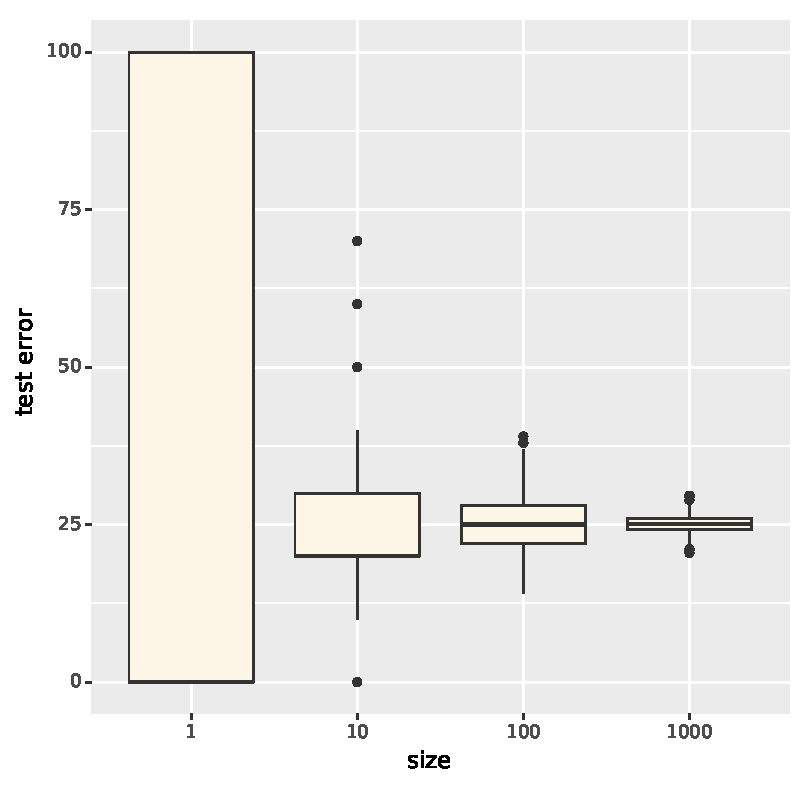
\includegraphics[scale=0.8]{test_error_fluctuations_1}\hspace*{0.5cm}
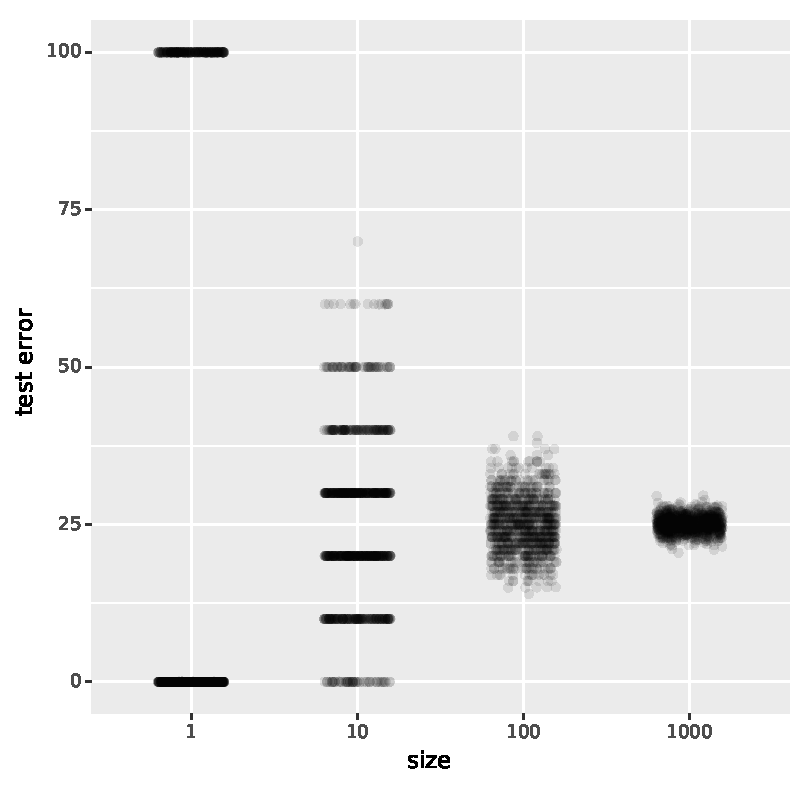
\includegraphics[scale=0.8]{test_error_fluctuations_2}}

\vspace*{-0.0cm}
$\triangleright$  depends on the dataset\\
$\triangleright$  statistical fluctuations decrease with size



\foilhead[-1cm]{Law of large numbers}

\textbf{Central limit theorem.}
Let $z_1, \ldots, z_N$ be independent and identically distributed samples form a \emph{real-valued distribution} with a \emph{finite standard deviation} $\sigma$ and \emph{mean} $\mu$. Then the random variable 
\begin{align*}
S=\sqrt{N}\Biggl(\frac{1}{N}\cdot \sum_{i=1}^N z_i -\mu\Biggr)
\end{align*}
converges \emph{in distribution} to normal distribution $\NNN(mean=0, sd=\sigma)$.  

\foilhead[-1cm]{Translation}


Under mild assumptions the empirical risk $R_N(f)$ converges to risk $R(f)$ and we can actually use normal distribution to estimate probabilities:
\begin{align*}
\pr{\abs{R_N(f)-R(f)}\geq \varepsilon} \lesssim 2\cdot \int\limits_{-\infty}^\varepsilon\frac{\sqrt{N}}{\sqrt{2\pi}\sigma}\exp{-\frac{N t^2}{2 \sigma^2}}dt
\end{align*}
for a finite value $\sigma$ where $\sigma^2$ is the variance of loss $\VAR(R(f))$.
\vspace*{1cm}

\textbf{Reasoning}
\begin{triangles}
\item If $(\vec{x}_i, y_i)$ are IID samples then $z_i=L(f(\vec{x}_i), y_i)$ are also IID samples.
\item By definition $\mu=\EXP(z)=\EXP(L(f(\vec{x}),y))=R(f)$.
\item CLT assumes that risk $\mu$ is finite and standard deviation $\sigma$ is finite.
\end{triangles}
\bigskip


\foilhead[-1cm]{Visual representation}

\illustration[scale=0.8]{normal_approximation}

\vspace*{-0.5cm}

Convergence implies that the centre area of is well approximated 
\begin{triangles}
\item 90\% confidence intervals are roughly the same for both distributions
\end{triangles}


\foilhead[-1cm]{Moment matching}

We know that the empirical risk $R_N(f)$ converges to normal distribution
\begin{triangles}
\item Normal distribution is fixed by a mean $\mu$ and variance $\sigma^2$
\item We can estimate mean $\hat{\mu}$ and variance $\hat{\sigma}^2$ of a loss term $L(f(\vec{x}), y)$ 
\item Then the estimates of mean and variance of the empirical risk are
\begin{align*}
\EXP(R_N(f))&\approx \hat{\mu}\\
\VAR(R_N(f))&\approx \frac{\hat{\sigma}^2}{N}
\end{align*}
\item This allows us to approximate $R_N(f)$ with normal distribution 
\end{triangles}



\foilhead[-1cm]{What does the convergence speed mean}

\begin{center}
\includegraphics[width=10cm]{sampling-bound-1}\hspace*{1cm}
\includegraphics[width=10cm]{sampling-bound-2}
\end{center}
\vspace*{-0.5cm}

The number of samples needed to get a precision $\varepsilon$ is $\Oh(1/\varepsilon^2)$. 
\begin{triangles}
\item To increase precision $10$ times you need $100$ times more samples!
\end{triangles}

\foilhead[-1cm]{Illustrative example}
\enlargethispage{1cm}
\illustration[scale=1.2]{perceptron_vs_conv_network_performanceover_folds}
\vspace{-3ex}
\begin{triangles}
\item Accuracy for 1000 element test sets
\item Accuracy estimetes vary more that the increase in the accuracy
\end{triangles}




\foilhead[-1cm]{Why do we need a test set at all}

\textbf{Machine learning algorithm}
\begin{triangles}
\item Count number of zeroes $n_0$ and number of ones $n_1$ in training sample.
\item If $n_0>n_1$ output $f_0(x)\equiv 0$, otherwise output $f_1(x)\equiv 1$.
\end{triangles}
\vspace*{1cm}

\textbf{Data source}
\begin{triangles}
\item Choose the input $x$ randomly form the range $[0,1]$
\item Choose the label $y$ randomly from the set $\set{0,1}$.
\end{triangles}

\vspace*{1cm}
\textbf{True risk value}
\begin{triangles}
\item Clearly the risk of both rules $R(f_0)=R(f_1)=0.5$.
\item The risk of of our learning algorithm $R(f)$ is also $0.5$. 
\end{triangles}

\foilhead[-1cm]{What happens during the training phase}

\illustration[scale=1.0]{empirical_risk_and_learning}

\begin{triangles}
\item We always choose the function $f_i$ that underestimates the true risk!
\item The probability that we go below the range effectively doubles. 
\end{triangles}


\foilhead[-1cm]{Simulation outcomes for other methods}

\illustration[scale=0.8]{training_bias_1}
\vspace*{-0.5cm}

Training error of the rule $f$ is significantly smaller than $0.5$.
\begin{triangles}
\item We bias the estimate by choosing the rule $g_i$ for which $R_N(f_i) < R(f)$.
\end{triangles}

\foilhead[-1cm]{Optimism}

\illustration[scale=0.8]{training_bias_2}
\vspace*{-0.5cm}
By knowing the \emph{optimism} $\Delta=R(f)-R_N(f_i$) we can correct $R_N(f)$.   
\begin{triangles}
\item Commonly mean value of $\Delta$ is used for the correction 
\end{triangles}


\foilhead[-1cm]{Optimism is only approximation}

\illustration[scale=0.8]{training_bias_3}
\vspace*{-0.5cm}
Optimism is usually anti-correlated with empirical risk $R_N(f)$   
\begin{triangles}
\item Simple shifting does not resolve the systematical bias  
\end{triangles}


\foilhead[0cm]{Why does the holdout testing work}

\illustration[scale=0.8]{holdout-design}

\

By randomly splitting the data into training and test data we assure
\begin{triangles}
\item The training and test sets are independent under IID assumption.
\item On a training set we compare many models and  choose few winners. 
\item These functions are independent from the test set data.
\item As there number of functions is small the law of large numbers holds. 
\end{triangles}


\foilhead[-1cm]{What is the right size of the holdout sample}

\illustration[width=10cm]{holdout-size}

The holdout sample must be quite large or otherwise the precision is low
\begin{triangles}
\item Roughly $400$ data points to get precision $0.1$ in classification accuracy.
\end{triangles}





\foilhead[-1cm]{Why is holdout testing problematic}

\begin{center}
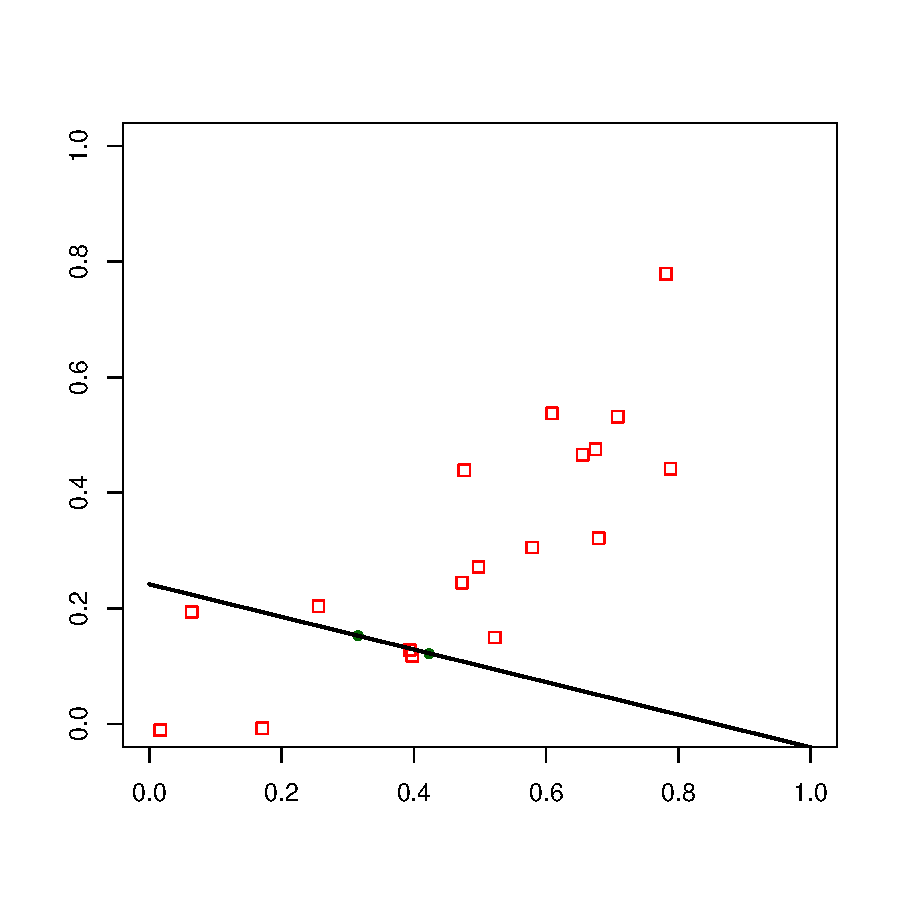
\includegraphics[width=10cm]{sample-split-1}\hspace*{1cm}
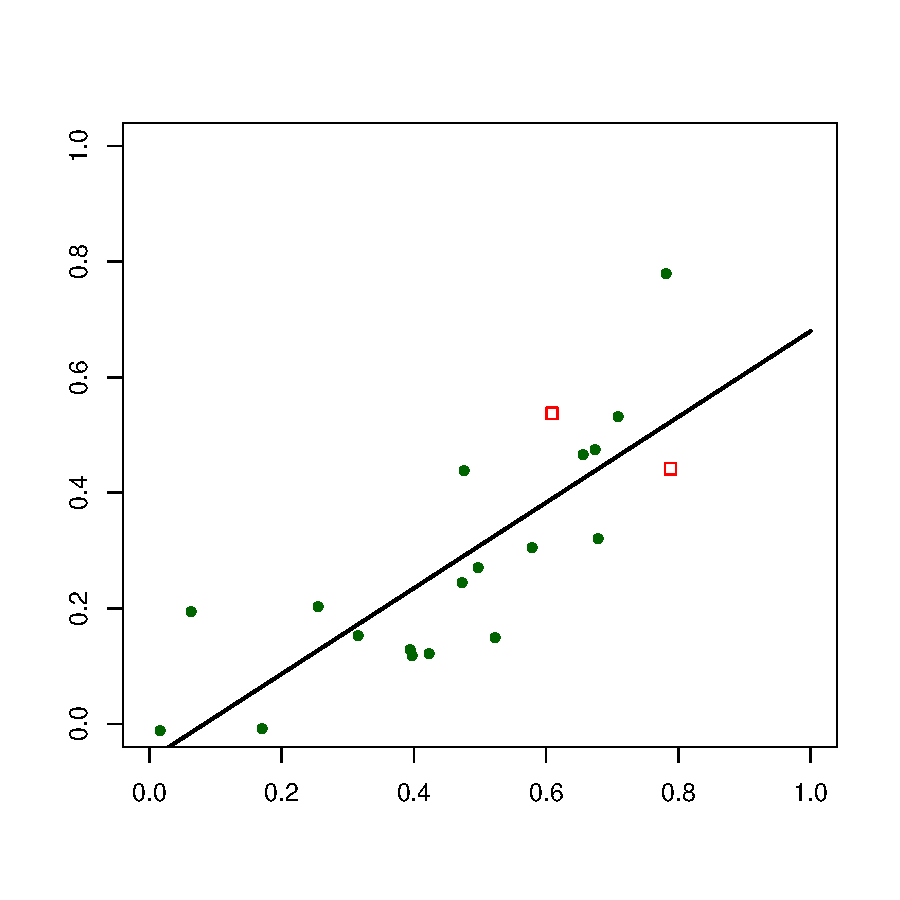
\includegraphics[width=10cm]{sample-split-2}
\end{center}
\vspace{-1cm}

If the number of available data points is small we have to choose:
\begin{triangles}
\item a small training set and bad model but good estimate on risk
\item a big training set and good model but bad estimate on risk
\end{triangles}

\foilhead[-1cm]{Why is holdout testing problematic}

\illustration[scale=0.8]{bias_variance_dilemma_1}
\vspace*{-.5cm}
Typical tradeoffs between learning-bias and variance of the validation error.   

\foilhead[-1.2cm]{Crossvalidation as an engineering trick}

\enlargethispage{0.7cm}

To reduce holdout error, we can do several holdout experiments. 
Since we do not have enough data, we redo splitting and training on the same data. 

This idea yields a generic crossvalidation scheme
\begin{enumerate}
\item Generate several splits of test and training data
\item For each split train the model and compute holdout error
\item Tabulate results\vspace*{2ex}
\begin{center}
\begin{tabular}{|l|c|c|c|c|}
\hline
 & Split $1$ & Split $2$ & $\ldots$ & Split $k$\\
 \hline
 Training error & $S_1$ & $S_2$ & $\ldots$ & $S_k$\\
 Test error     & $E_1$ & $E_2$ & $\ldots$ & $E_k$\\
\hline
 Optimism $\Delta$    & $E_1-S_1$ & $E_2-S_2$ & $\ldots$ & $E_k-S_k$\\
 \cline{2-5}
\hline
\end{tabular}
\end{center}
\vspace*{2ex}
\item Compute averages $E=\frac{1}{k}(E_1+\cdots+E_k)$ and $\Delta=\frac{1}{k}(\Delta_1+\cdots+\Delta_k)$
\item Visualise results and compute confidence intervals for estimates if needed. 
\end{enumerate}

\foilhead[-0.5cm]{How many splits should we take?}

\illustration[scale=0.9]{crossvalidation_and_moment_matching}

Moment matching provides variability estimates for cross-validation. 
\begin{triangles}
\item Resulting bounds are incorrect and underestimate the error.
\item The main reason is the correlation between splits.   
\end{triangles}


\foilhead[-1cm]{What does crossvalidation measure?}

For each fold we have a separate predictor $f_i$ and test error $E_i$:
\begin{triangles}
\item Average $E$ characterises average behaviour of $f_1,\ldots, f_k$.
\item Algorithm can use only (1-1/k) fraction of the available data.
\item If there is not enough data for training $E$ overestimates the error. \vspace*{1cm}  
\end{triangles}

To estimate the performance of a classifier $f$ trained on the entire data:
\begin{triangles}
\item We must estimate the difference between test and training error $\Delta(f)$.
\item For normal ML algorithm optimism decreases by increasing the size $n$.
\item Crossvalidation estimates $\Delta$ at the point $(1-1/k)\cdot n \lesssim n$. 
\item Hence we can go from training error to test error estimate.
\item Training and test set fluctuations influence the outcome.  
\end{triangles}
 

\foilhead[-1cm]{Crossvalidation vs holdout estimates}

\illustration[scale=0.8]{crossvalidation_vs_holdout}
\vspace*{-.5cm}
\begin{triangles}
\item Crossvalidation error is slightly larger as the training set is smaller.  
\item Crossvalidation error is slightly more fluctuating due to correlations. 
\item Quite often these effects are quite small in practice. 
\end{triangles}



\foilhead[-1cm]{Theoretical explanation}

\textbf{Theorem.} 
Crossvalidation error $E =\frac{1}{k}(E_1+\cdots+E_k)$ is an 
unbiased estimate for the average test error that is taken over all models that are trained on $(1-1/k)\cdot n$ samples. 

\textbf{Proof}
\begin{align*}
\EXP[E] =\frac{\EXP[E_1]+\cdots+\EXP[E_k]}{k}=\EXP_{tr}\biggl[\EXP_{\vec{x}, y}\bigl[L(f(\vec{x}),y)|f=\AAA(train)\bigr]\biggr]
\end{align*}
where 
\begin{triangles}
\item the outer expectation is taken over all possible training sets  
\item the inner expectation measures the risk of the fitted model
\end{triangles}


\foilhead[-1cm]{Crossvalidation variance estimate}

\centerline{
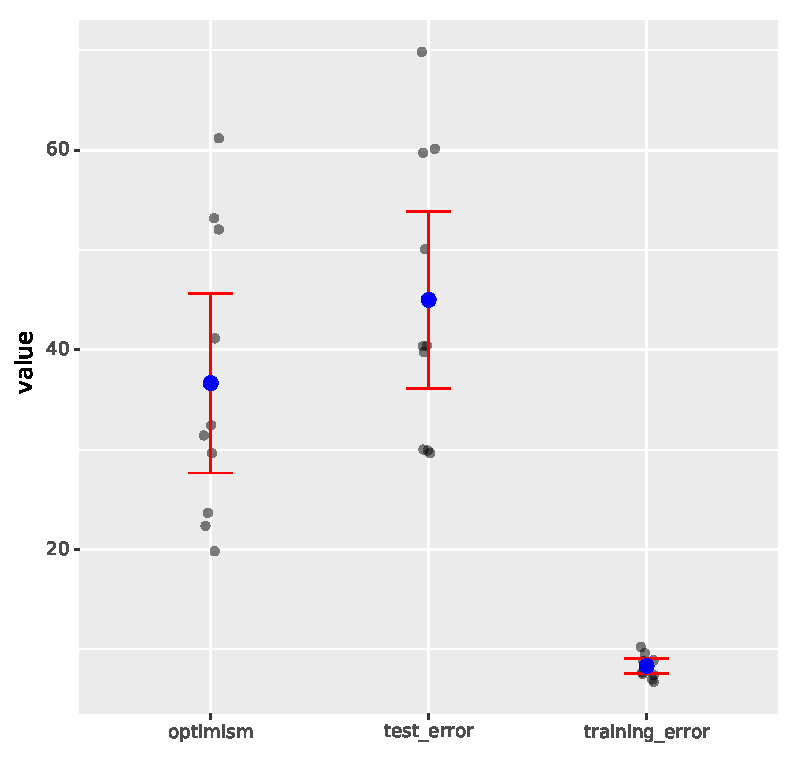
\includegraphics[scale=0.8]{crossvalidation_moment_matching}\hspace*{0.5cm}
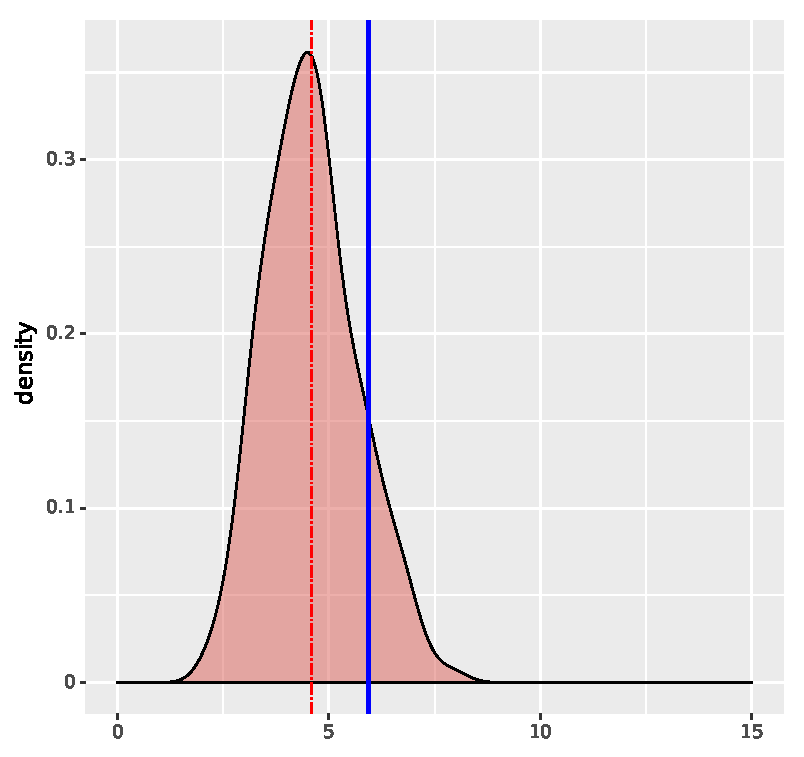
\includegraphics[scale=0.8]{crossvalidation_variance_estimate}}
\vspace*{-.5cm}
\begin{triangles}
\item The naive variance estimate for the crossvalidation error is biased.   
\item The estimate usually gives smaller confidence intervals as they are.  
\item This must be accounted in the estimates of optimism and test error. 
\end{triangles}



\foilhead[-1cm]{Theoretical explanation}

\textbf{Theorem.}
The variance of crossvalidation error $E =\frac{1}{k}(E_1+\cdots+E_k)$ is a weighted average consisting of three components
\begin{align*}
\theta = \frac{1}{n}\cdot\sigma^2+\textcolor{red}{\frac{m-1}{n} \cdot\omega + \frac{n-m}{n}\cdot\gamma}
\end{align*} 
where
\begin{triangles}
\item $m$ is the number of samples in each fold, i.e., $m\approx n/k$. 
\item $\sigma^2$ is the average variance of true test examples.
\item $\omega$ is the within-block covariance of test errors sharing the same test set. 
\item $\gamma$ is the between-block covariance of test errors cause by the fact that 
\begin{diamonds}
 \item training set have large intersection
 \item test fold is inside the training set of another split. 
\end{diamonds}   
\end{triangles}

 





\foilhead[-1cm]{What else can we do with crossvalidation?}

\textbf{Comparing different algorithms}
\begin{triangles}
\item We can tune hyperparameters of the algorithm
\item We can estimate which algorithm on average behaves better
\item We can quantify the stability of the performance ranking\vspace*{0.5cm}
\end{triangles} 

\textbf{Estimating variance of model parameters}
\begin{triangles}
\item Different folds give different parameter instances
\item Parameter confidence intervals can be used for diagnostics
\item Confidence intervals can be used for pruning spurious coefficients\vspace*{0.5cm}
\end{triangles} 

\textbf{Finding hard instances}
\begin{triangles}
\item Different folds give different mismatches $\hat{y}_i\neq y_i$
\item Corresponding problem instances $(\vec{x}_i, y_i)$ can be studied further
\end{triangles}


\foilhead[-1cm]{Estimating variance of model parameters}

\centerline{
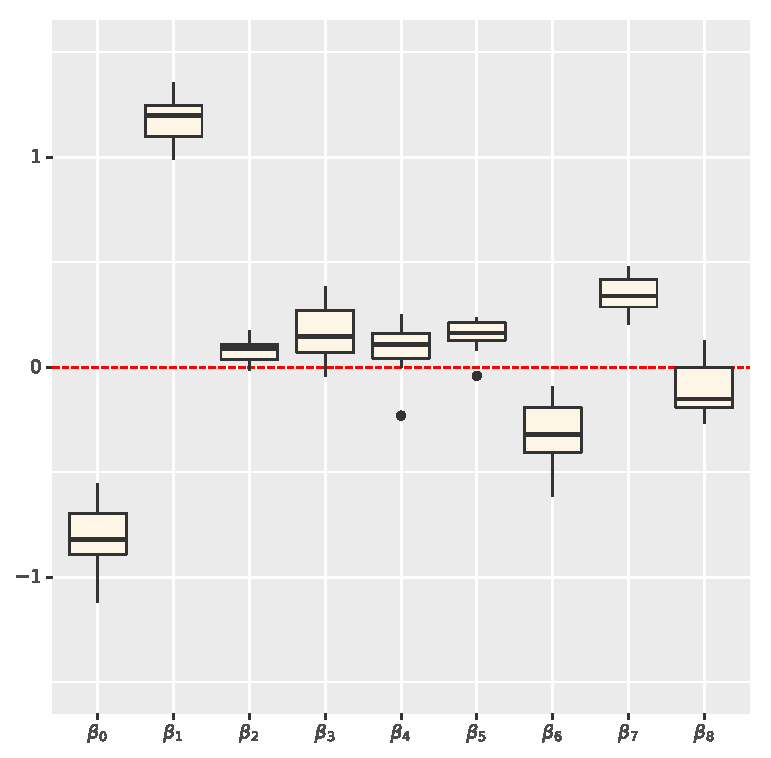
\includegraphics[scale=0.8]{crossvalidation_parameter_variance_i}\hspace*{0.5cm}
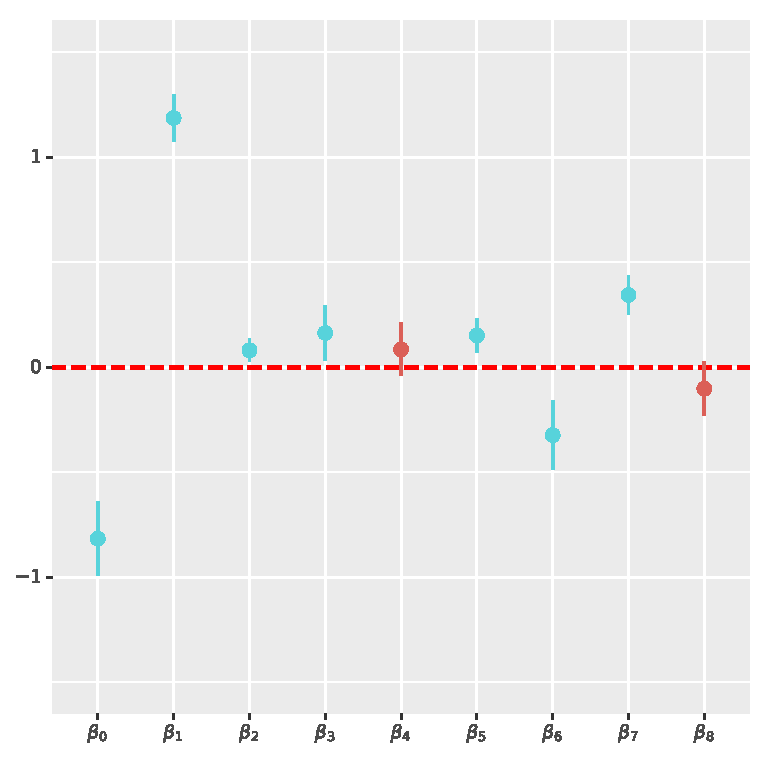
\includegraphics[scale=0.8]{crossvalidation_parameter_variance_ii}}
\vspace*{-.5cm}
\begin{triangles}
\item The method is applicable for models with compact parametrisation.
\item Each split defines a new model $f_i$ with coefficient $\vec{\beta}$.   
\item The variability of a coefficient $\beta_i$ shows its certainty and relevance. 
\end{triangles}


\foilhead[-1cm]{Other flavours of cross validation}

\textbf{Exhaustive data splitting}
\begin{triangles}
\item Leave-one-out method, leave-$p$-out method
\end{triangles}
\vspace*{1cm}

\textbf{Partial splitting}
\begin{triangles}
\item $K$-fold cross validation for $K = 5 , 10$ 
\item Monte-Carlo crossvalidation with a fixed split ratio, e.g $1:9$.\\ Same split can occur more than once  
\item Repeated learning testing with  a fixed split ratio, e.g $1:9$.
\\ Same split can occur only once. 
\end{triangles}


\foilhead[-1cm]{Bootstrapping as an alternative}

We could use the entire date set for validation if we could get another dataset for training the model. Bootstrapping is an engineering trick to create a new dataset out of a thin air.
\begin{enumerate}
\item Draw $N$ samples from the original dataset with replacement to get a \emph{bootstrap sample} $D_{B}$, e.g. the same element can occur more than once.
\item Train the model  on the bootstrap sample $D_B$.
\item Estimate the test error on the original dataset $D$.
\item Repeate the procedure $20$-$200$ times.
\item Compute necessary statistics and visualise the results if needed.
\end{enumerate}


\foilhead[-1cm]{Standard way how to use bootstrapping}
 
Bootstrapping is mostly used to estimate optimism
\begin{triangles}
\item The model is trained and the training error $S_i$ is computed.
\item The test error $E_i$ is usually computed on the entire dataset.
\item Optimism is computed as $E_i-S_i$.
\end{triangles}

\bigskip

Note that it does not make sense to compute test error on the entire dataset as we have used some of the data to build a model. Advanced bootstrap methods like \textbf{.632 bootstrap} and \textbf{.632 bootstrap+} use only the out of training set error and later find a tradeoff between training an test error.
\begin{align*}
E_{\text{boot}}=0.368\cdot S_{\text{Train}} + 0.632\cdot E_{\text{Out-of-training-set}}
\end{align*}

\foilhead[-1cm]{Other uses of bootstrapping}

Estimate the noise-tolerance of the machine learning method
\begin{triangles}
\item Generate a bootstrap sample.
\item Corrupt with an appropriate noise.
\item Train the model and estimate the performance.
\end{triangles}
\vspace*{2cm}

Estimate the variance of model coefficients
\begin{triangles}
\item Generate a bootstrap sample.
\item Estimate model parameters.
\item Visualise parameters and compute empirical quantiles.
\item Drop parameter which fluctuate around zero.
\end{triangles}

\end{document}
